\section{Mass Spectrometry}
A mass spectrometer (MS) is a device used to measure the mass to charge ratio (m/z) of ions.
Usually, this charge to mass ratio is calculated from either how much an ion is deflected in a magnetic field or accelerated in an electric field – ions with the same ratio are deflected/accelerated equally.
This information can be used for a variety of purposes such as determining an unknown isotope in a mixture or to directly measure nuclear masses.

\subsection{Importance to mass spectrometry}
Mass spectrometer is integral to nuclear theory study for identifying or quantifying unknown samples (ions) as well as measuring binding energy of a particle to gain information about its nuclear structure.
Nuclear mass is a fundamental property which has been responsible for the discovery of many nuclear effects such as shell closures and nucleon-nucleon pairing.
[2] MS are used in nuclear physics research to explore exotic nuclei (such as neutron rich calcium isotopes) and isotopes with high neutron to proton ratios are interesting to study as they can develop our understanding of nuclear forces.
Examining this excess mass “defect” is the most important metaphor of nuclear physics: “the valley of stability” which has the lowest mass excess.
Overweight nuclides that farther away from equilibrium tend to have their mass excess with much shorter half-lives which is defined by the binding energy.

The charge to mass ratio was first measured by J. J. Thomson in the late 19th century [3] and throughout the 20th century MS have evolved with numerous variations and different set ups.
This report focused on 2 types of MS: the Penning trap and the Multiple Reflector Time of-Flight mass spectrometer (MR-TOF), as both are currently used to measure the mass of exotic nuclei.[4]

\subsection{How a general MS works}
In general MS have three main components: an ioniser, mass analyser and a detector.
A sample must be ionised before entering the mass analyser so it will interact with the magnetic and/or electric fields.
In the mass analyser the beam is accelerated/deflected before being incident on a detector.
The detector then measured the mass charge ratio based on the time or location of incidence.
5] Ionization methods including thermal ionization and electron impact ionization are used.
Sample was heated floating around the tube and beamed or bombarded with a bunch of electrons, which can knock off electrons from the atoms in my sample to ionize them.
At the end of chamber there is a detector usually are electron multiplier like faradays cup, measuring quantity and time of arrival.
The more the ions hit a certain part of the detector it means the sample has more of that type of isotope in nature.
And from all that, MS can generate the spectrum which is useful for analysing unknown samples.

\subsection{Penning traps}
Penning traps are the most common development with their currently being 7 active laboratories including CPT, ISOLTRAP, JYFLTRAP, LEBIT, SHIPTRAP, TITAN and they also give us the most precise measurement for stable isotopes.
Just 15 years ago, the only penning trap spectrometer publishing the masses of radioactive samples was the pioneering experiment ISOLTRAP, set up at CERN’s ISOLDE facility in 1986.
Penning traps are based on a cyclotron design, and they trap the isotopes using a combination of strong longitudinal uniform magnetic and quadrupole electric fields, a high homogeneity also reduces the possibility to field drifts so that they move periodically and then the frequency is related to mass following the equation
\begin{equation}
    \nu_c = \frac{1}{2\pi}\frac{qB}{m}
\end{equation}
the measured quantity is cyclotron frequency which can be essentially measured in high accuracy.
Also, the coexistence of trapping and cooling minimizes systematic errors from mass measurement though the time it takes to complete a cycle is the main limitation of mass measurement which tends to limit the range of isotopic species that can be measured.

\begin{figure}[H]
    \centering
    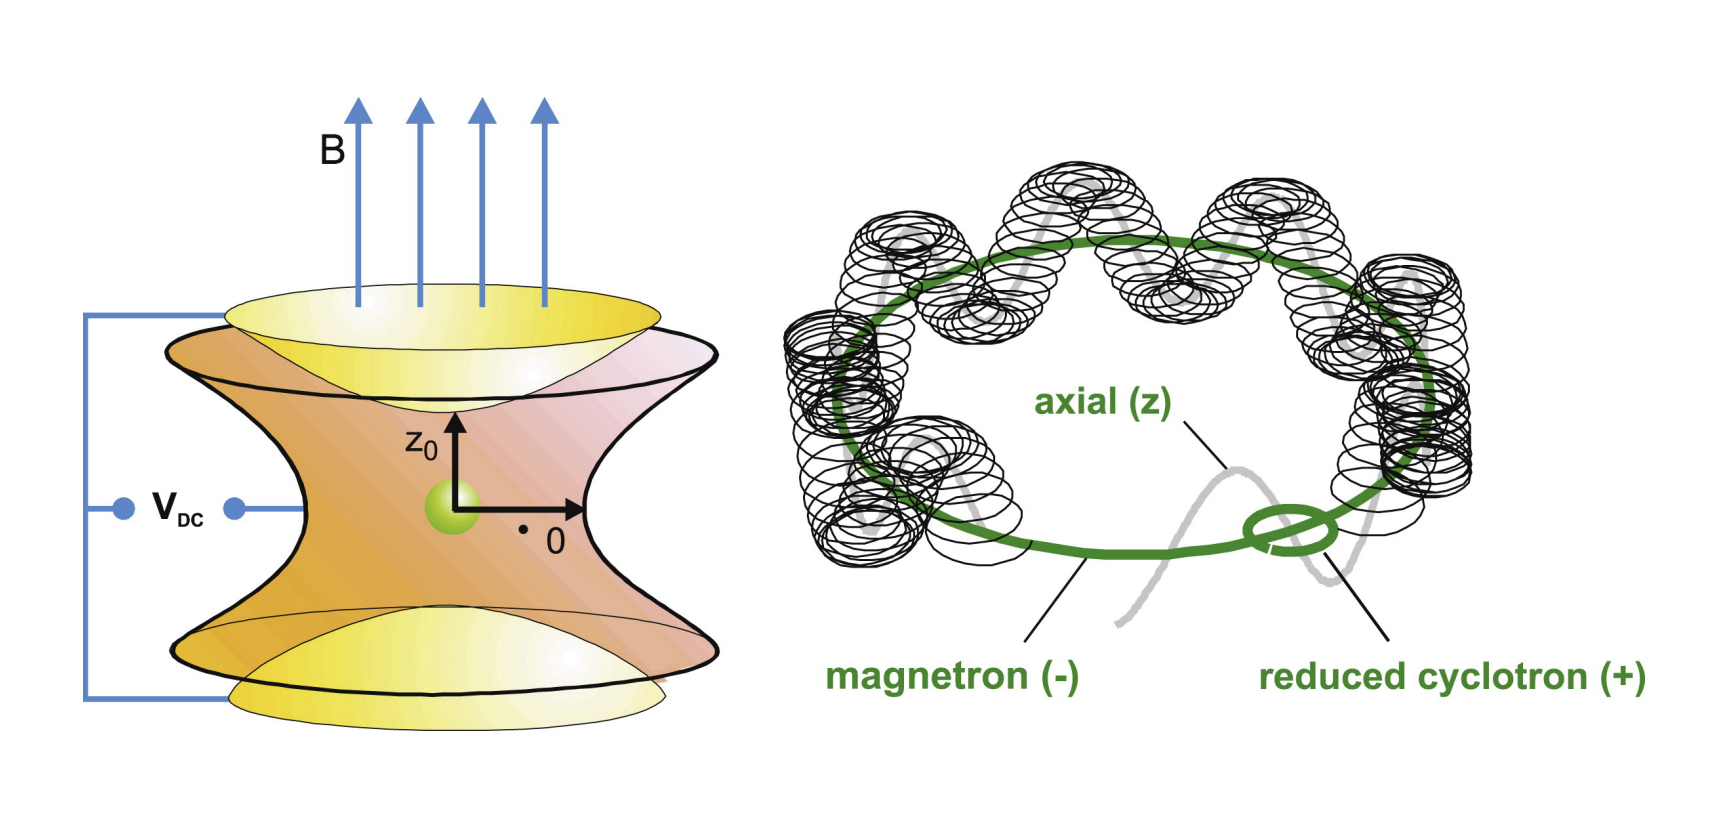
\includegraphics[width=.4\textwidth]{images/MS_penningtrap.png}
    \caption{Schematic diagram of a Penning trap.}\label{fig:MS_PT}
    % Most models predict many more yet unmeasured nuclei in the white zone, mostly under the visible data and a above what's called the neutron drip line (not shown in the plot).\cite{erler_limits_2012}}
    % According to most predictions there could be once as many very unstable nuclei yet unmeasured (in the white zones).}
\end{figure}

\subsection{MR-TOF mass spectrometers}
MR-TOF devices are the newest ion-trap improvement, first being used in 2013, they are often used accompanied with penning traps.
Their greatest advantage is that they can provide measurements for isotopes with very low production rates and very short half-lives, which is particularly suitable for short lived nuclei as they can resolve in less than 30ms and suited to rare nuclei as they can resolve small sample sizes.
MR-TOF works by reflecting the ions back and forth between two electrostatic mirrors in a short tube, effectively increasing the flight path length.
The key is that the speed inside depends on the mass-to-charge ratio, so after a while, the isotopes are released, and the mass is calculated from the timing through this equation
\begin{equation}
    t = \frac{d}{\sqrt{2U}}\sqrt{\frac{m}{q}}
\end{equation}

MR-TOF is usually faster and more sensitive as a non-scanning device with high ultra-mass resolving power than a penning trap.
It has several advantages compared to a frequency-based mass spectrometer also including the single-ion sensitivity, short cycle time (5ms) and superior resolving power for a measurement time of 1s and mass-to-charge ratio larger than hundreds of u.
